\documentclass[a4paper, 12pt]{article}

\newcommand\tab[1][.6cm]{\hspace*{#1}}
\usepackage[portuges]{babel}
\usepackage[utf8]{inputenc}
\usepackage{amsmath}
\usepackage{mathtools}
\usepackage{indentfirst}
\usepackage{graphicx}
\usepackage{multicol,lipsum}
\usepackage{blindtext}
\usepackage{verbatim}
\usepackage{textcomp}
\usepackage{hyperref}
\usepackage{float}
\usepackage{url}

\begin{document}
%\maketitle

\begin{titlepage}
	\begin{center}
	
	\begin{figure}[ht]
    \centering
    
\includegraphics[width=.44\textwidth]{Images/LogoUFSJ.PNG}
    \label{fig:Capturar.PNG}
    \end{figure}

    	\Huge{Universidade Federal São João del Rei}\\
		\Large{Curso de Ciência da Computação}\\ 

        \vspace{110pt}
        \textbf{\LARGE{
        \\
        \\
        \\
        Exercícios Avaliativos\\
        \vspace{0.5cm}
        \Large{Introdução à Modelagem Computacional}
        \\
        \\
        \\
        }}
        
		\title{{\large{Título}}}
		\vspace{2.5cm}
	\end{center}
	    
    \begin{flushleft}
		\begin{tabbing}
		\\
		\\
		\\	
		\large{Discente: Julio Cesar da Silva Rodrigues}\\
	    \\
		\large{Docente: Alexandre Bittencourt Pigozzo}\\
	    \end{tabbing}
    \end{flushleft}
	\vspace{1cm}
	
	\begin{center}
		\vspace{\fill}
			Maio\\
		    2023
	\end{center}
\end{titlepage}

\section*{Exercício 1}

O modelo construído utilizando a ferramenta \emph{Insight Maker} que representa a ocorrência das reações é exibido na Figura \ref{fig:exampleFig1}

\begin{figure}[H]
    \centering
    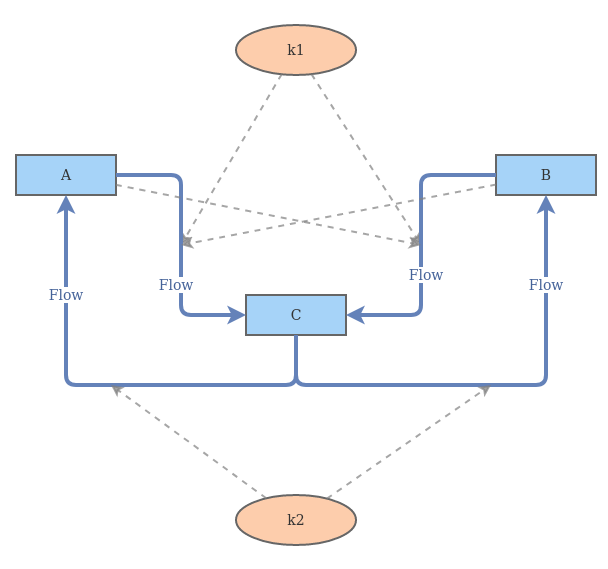
\includegraphics[width=1\textwidth]{Images/Exercise 1/model.png}
    \caption{Modelo de Reações Químicas}
    \label{fig:exampleFig1}
\end{figure}

Foi criado um conjunto de \emph{stocks} representando as moléculas hipotéticas que correspondem as populações A, B e C (e seus níveis de concentração).

Foram criados dois fluxos direcionados para C, e ambos possuem a mesma modelagem do número de reações, multiplicando a taxa \emph{\(k_1\)} pelas concentrações de A e B ao longo do tempo, produzindo C.

\begin{align*}
    \frac{dA}{dt} = k_1 \cdot A \cdot B \hspace{1cm}
    \frac{dB}{dt} = k_1 \cdot A \cdot B
\end{align*}

De forma semelhante, foram criados dois fluxos para representar a reação de volta, desta vez com uma taxa \(k_2\) com que a concentração de moléculas de C "derivam" A e B, aumentando suas concentrações.
\begin{align*}
    \frac{dC}{dt} = k_2 \cdot C
\end{align*}

Uma simulação\(^*\) inicial foi realizada (Figura \ref{fig:exampleFig2}), utilizando as condições iniciais à seguir:

\begin{itemize}
    \item \(A = 2\)
    \item \(B = 1\)
    \item \(C = 0\)
    \item \(k_1 = 0.1\)
    \item \(k_2 = 0.05\)
\end{itemize}

\begin{figure}[H]
    \centering
    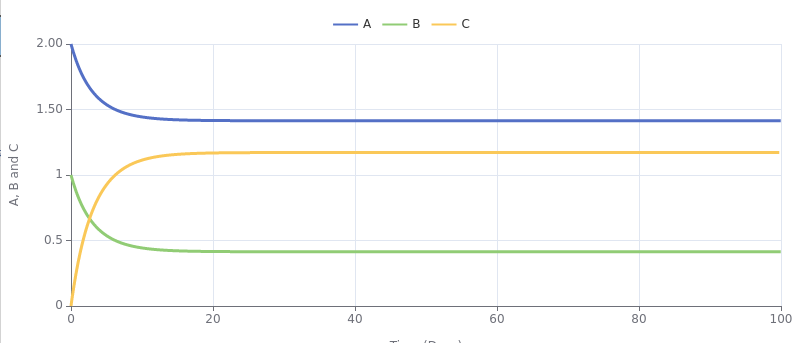
\includegraphics[width=1\textwidth]{Images/Exercise 1/vanilla.png}
    \caption{Reações Químicas ao Longo do Tempo}
    \label{fig:exampleFig2}
\end{figure}

\noindent * Todas as simulações deste exercício foram realizadas com passo de tempo 0,01 e mensurado em dias.

\subsection*{Alterando Parâmetros, Condições Iniciais e Análises}

Para o parâmetro \(k_1\), foi observado que elevações em seu valor implicam no aumento da concentração de C em relação as concentrações de A e B, que se mostram inferiores como é mostrado na Figura \ref{fig:exampleFig3}. As condições iniciais da simulação são detalhadas à seguir:

\begin{itemize}
    \item \(A = 2\)
    \item \(B = 1\)
    \item \(C = 0\)
    \item \(k_1 = 1\)
    \item \(k_2 = 0.05\)
\end{itemize}

\begin{figure}[H]
    \centering
    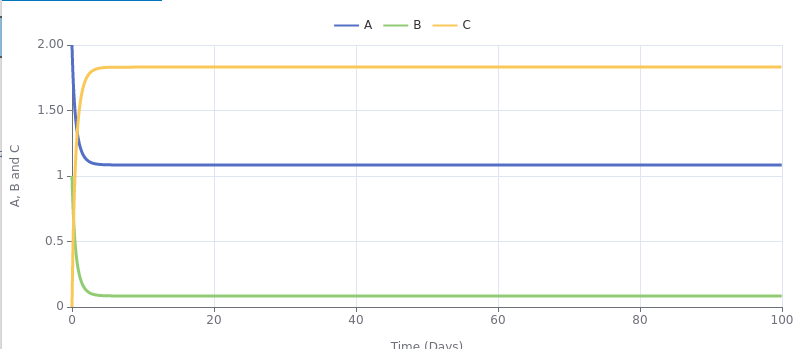
\includegraphics[width=1\textwidth]{Images/Exercise 1/k1.png}
    \caption{Reações Químicas ao Longo do Tempo Variando \(k_1\)}
    \label{fig:exampleFig3}
\end{figure}

Em contrapartida, atribuindo valores muito baixos para \(k_1\) produzem um efeito inverso, com C apresentando uma concentração menor em relação as concentrações de A e B ao longo do tempo na simulação.

Para o parâmetro \(k_2\), foi observado que elevações em seu valor implicam em pouco decréscimo nas concentrações de A e B, enquanto o crescimento de C se mostra relativamente discreto, com concentração final inferior as de A e B como é mostrado na Figura \ref{fig:exampleFig4}. As condições iniciais da simulação são detalhadas à seguir:

\pagebreak

\begin{itemize}
    \item \(A = 2\)
    \item \(B = 1\)
    \item \(C = 0\)
    \item \(k_1 = 0.1\)
    \item \(k_2 = 0.5\)
\end{itemize}

\begin{figure}[H]
    \centering
    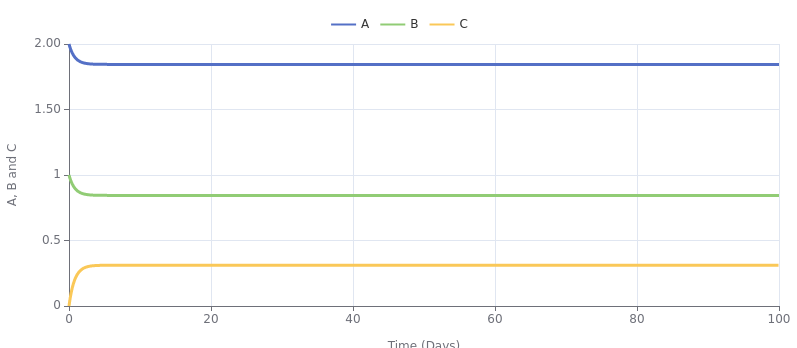
\includegraphics[width=1\textwidth]{Images/Exercise 1/k2.png}
    \caption{Reações Químicas ao Longo do Tempo Variando \(k_2\)}
    \label{fig:exampleFig4}
\end{figure}

Além disso, a atribuição de valores muito baixos para \(k_2\) produzem um efeito ainda mais discrepante, com C apresentando uma crescimento quase desprezível em relação as concentrações de A e B ao longo do tempo na simulação.

Em resumo, para as condições iniciais em que as concentrações de A e B são superiores a de C, valores extremos de \(k_1\) aceleram ou inibem o aumento da concentração de C e decréscimo nas concentrações de A e B. Valores extremos de \(k_2\) tendem a estagnar rapidamente as concentrações de A e B ao longo do tempo e inibir proporcionalmente a produção de C.

Por fim, foi realizada uma última simulação (Figura \ref{fig:exampleFig5}), desta vez com a concentração inicial de C superior às concentrações de A e B, sem alterar as taxas iniciais de \(k_1\) e \(k_2\). O resultado obtido foi o esperado, com a concentração de C apresentando decréscimo, e as concentrações de A e B apresentando crescimento, uma situação inversa à aquela observada na primeira simulação. As condições iniciais da simulação são detalhadas à seguir:

\begin{itemize}
    \item \(A = 1\)
    \item \(B = 0\)
    \item \(C = 3\)
    \item \(k_1 = 0.1\)
    \item \(k_2 = 0.05\)
\end{itemize}

\begin{figure}[H]
    \centering
    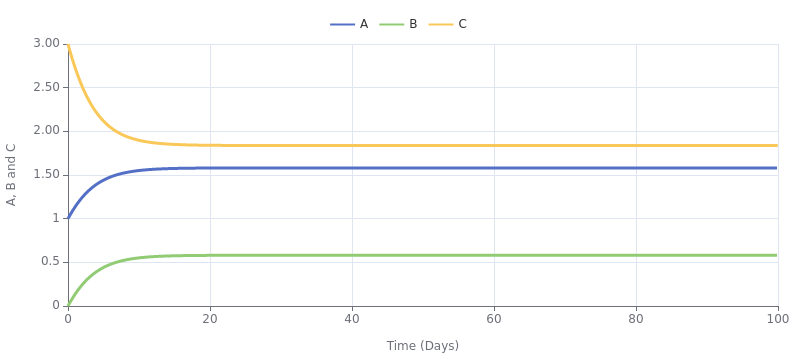
\includegraphics[width=1\textwidth]{Images/Exercise 1/c.png}
    \caption{Impacto das Condições Iniciais na Simulação}
    \label{fig:exampleFig5}
\end{figure}

\section*{Exercício 2}

Para a modelagem de cada uma das EDOs, assume-se como significado de cada variável:

\begin{itemize}
    \item \(A\): Concentração de moléculas do tipo A;
    \item \(B\): Concentração de moléculas do tipo B;
    \item \(C\): Concentração de moléculas do tipo C;
    \item \(k_1\): Probababilidade da reação (síntese) entre duas moléculas quaisquer A e B para produzir C (A + B $\xRightarrow{k_1}$ C);
    \item \(k_2\): Probababilidade da reação (decomposição) de uma molécula qualquer C para produzir A e B (C $\xRightarrow{k_2}$ A + B).
\end{itemize}

\subsection*{Reação com A e B}
\begin{align*}
    \frac{dA}{dt} & = - k_1 \cdot A \cdot B + k_2 \cdot C\\
    \\ \frac{dB}{dt} & = - k_1 \cdot A \cdot B + k_2 \cdot C
\end{align*}

Como apenas existe uma única reação entre A e B de forma conjunta, é utilizada a mesma EDO para modelar suas concentrações ao longo do tempo. O termo \(-k_{1}AB\) representa o decréscimo (sinal negativo) nas concentrações de A e B com uma taxa \(k_1\), conforme a ocorrência das reações. Já o termo \(k_{2}C\) ,representa o aumento (sinal positivo) na concentração de moléculas do tipo C, com uma taxa \(k_2\) à medida que as reações ocorrem, com A e B derivando C (reação de síntese).

\subsection*{Reação com C}
\begin{align*}
    \frac{dC}{dt} & = k_1 \cdot A \cdot B - k_2 \cdot C
\end{align*}

O termo \textbf{\(k_{1}AB\)} representa o aumento (sinal positivo) nas concentrações de A e B com uma taxa \(k_1\), conforme a ocorrência das reações. Já o termo \(-k_{2}C\), representa o decréscimo (sinal negativo) na concentração de moléculas do tipo C, com uma taxa \(k_2\) à medida que as reações ocorrem, com C decompondo-se em A e B (reação de decomposição).

\subsection*{Resultados}

Por fim, foram realizadas simulações utilizando os mesmos parâmetros explorados no modelo sintetizado na plataforma \emph{Insight Maker} para testar o funcionamento correto, e principalmente, a concordância entre resultados para investigar possíveis incoerências. Os resultados obtidos foram extremamente parecidos com aqueles sumarizados pelos gráficos apresentados nas Figuras \ref{fig:exampleFig2}, \ref{fig:exampleFig3}, \ref{fig:exampleFig4} e \ref{fig:exampleFig5} (inclusive as análises).

Para efeitos de comparação e checagens, os resultados obtidos com o modelo desenvolvido em linguagem \emph{Python} são exibidos nas Figuras \ref{fig:exampleFig6}, \ref{fig:exampleFig7}, \ref{fig:exampleFig8} e \ref{fig:exampleFig9}:

\begin{figure}[H]
    \centering
    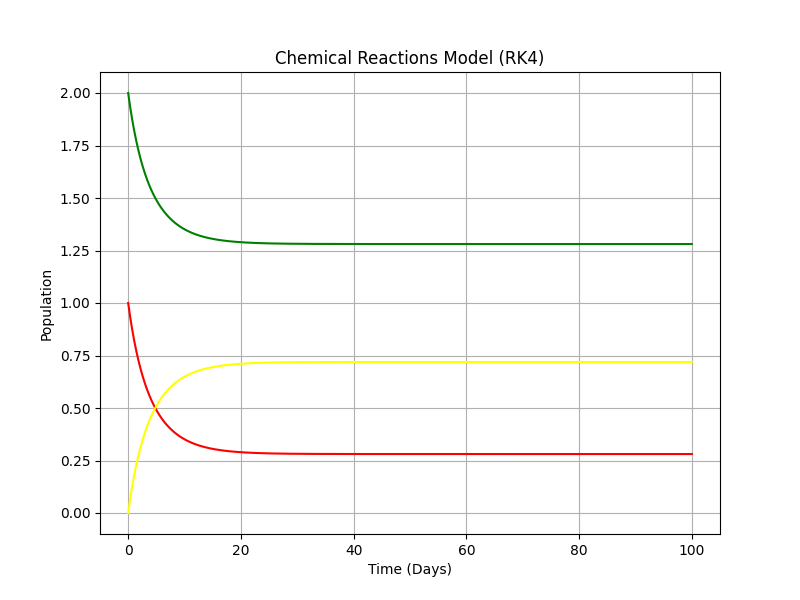
\includegraphics[width=0.88\textwidth]{Images/Exercise 2/vanilla.png}
    \caption{Reações Químicas ao Longo do Tempo}
    \label{fig:exampleFig6}
\end{figure}

\begin{figure}[H]
    \centering
    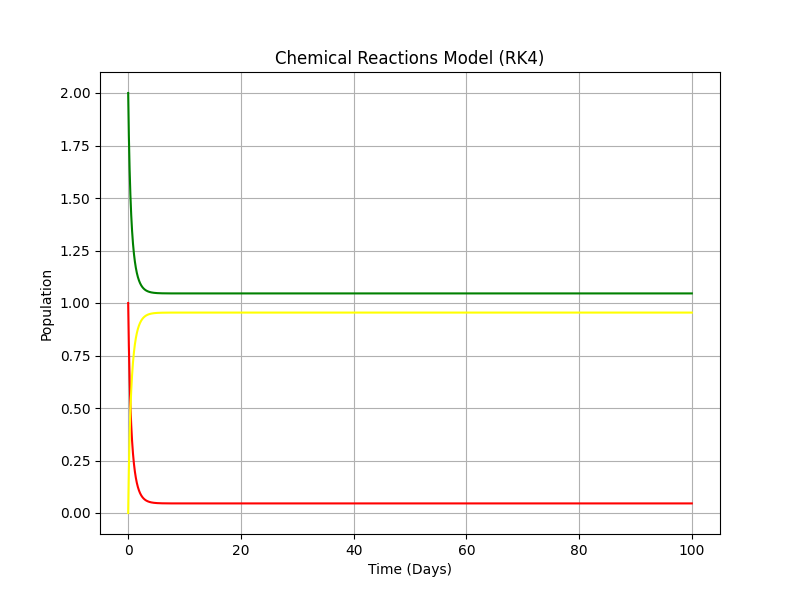
\includegraphics[width=0.88\textwidth]{Images/Exercise 2/k1.png}
    \caption{Reações Químicas ao Longo do Tempo Variando \(k_1\)}
    \label{fig:exampleFig7}
\end{figure}

\begin{figure}[H]
    \centering
    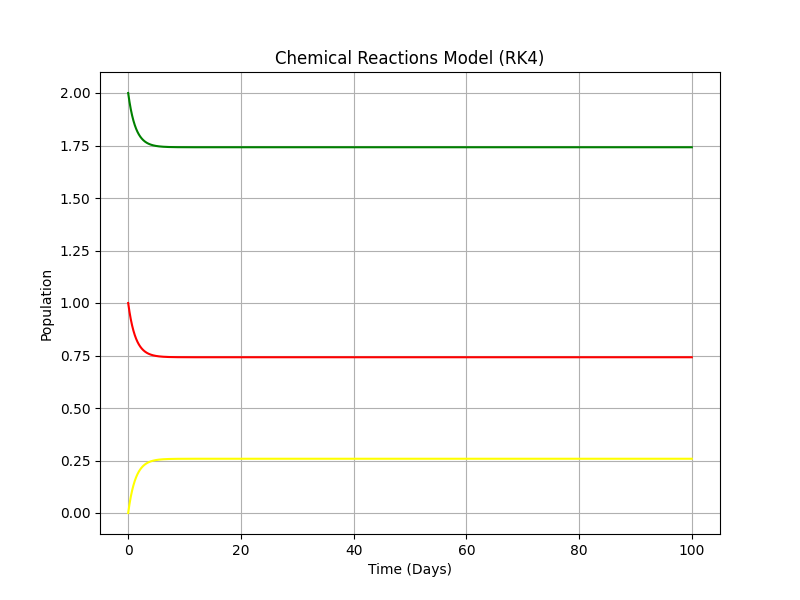
\includegraphics[width=0.88\textwidth]{Images/Exercise 2/k2.png}
    \caption{Reações Químicas ao Longo do Tempo Variando \(k_2\)}
    \label{fig:exampleFig8}
\end{figure}

\begin{figure}[H]
    \centering
    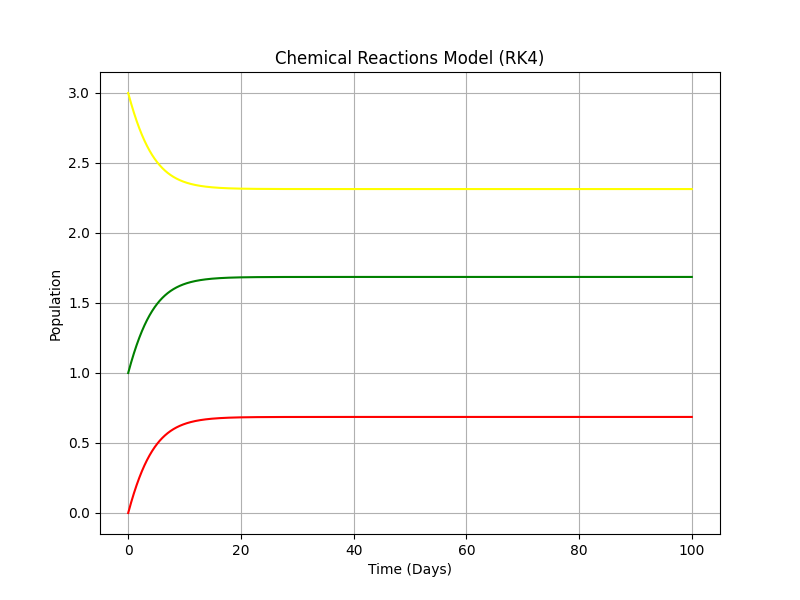
\includegraphics[width=0.88\textwidth]{Images/Exercise 2/ic.png}
    \caption{Impacto das Condições Iniciais na Simulação}
    \label{fig:exampleFig9}
\end{figure}

\section*{Exercício 3}

To be continued...

\section*{Exercício 4}
\section*{Exercício 5}
\section*{Exercício 6}

\pagebreak

\section*{Referências}

\begin{itemize}
    \item Repositório com implementações de métodos e modelos do docente da disciplina: \url{https://github.com/alexbprr/ComputationalModeling};
    \item Material disponível no portal didático na disciplina de Introdução à Modelagem Computacional.
\end{itemize}

\end{document}